\chapter{Interface K8s Cluster and GitLab-OST}

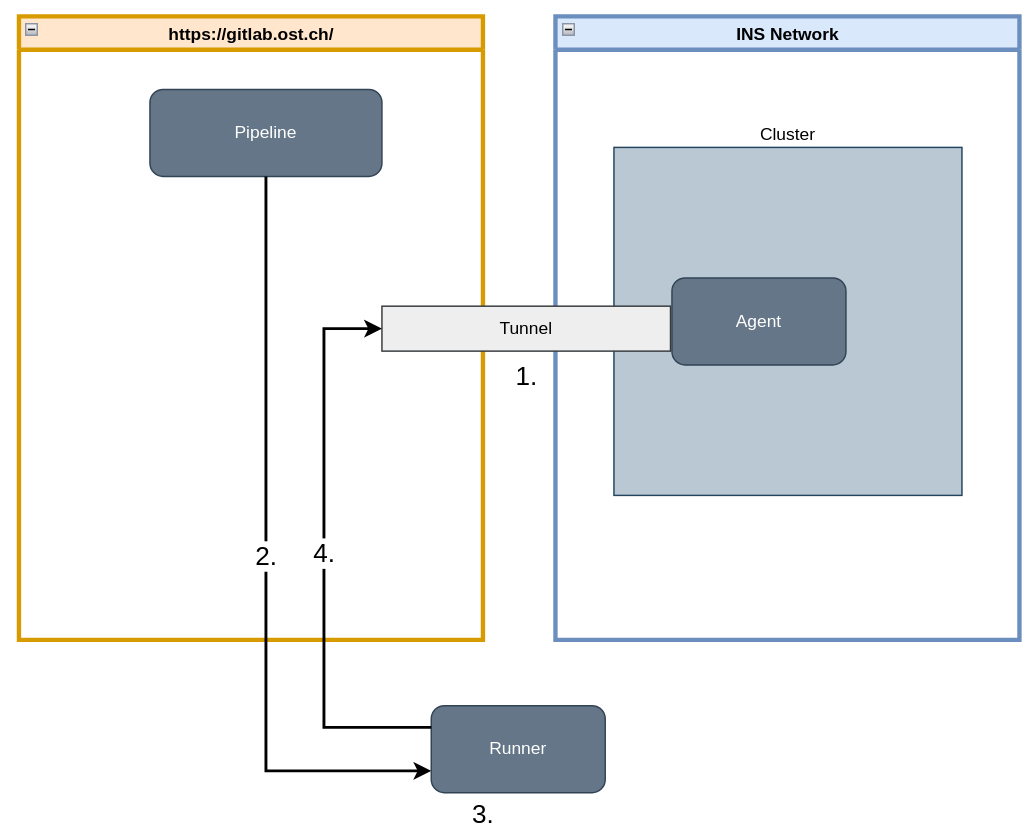
\includegraphics[height=12cm]{resources/k8s_including_in_gitlab-ost.png}
\begin{enumerate}
    \item The \textit{Agent} create a \textit{Tunnel} from the INS network to the gitlab.ost.ch network.
    \item The \textit{Pipeline} trigger the \textit{Runner} to run the cluster commands.
    \item The \textit{Runner} start the docker.
    \item The \textit{Runner} get via the gitlab.ost.ch network access to the \textit{tunnel endpoint} and run the cluster commands now at the cluster.
\end{enumerate}

The figure above shows you how the Kubernetes cluster and the GitLab are combined. The GitLab and the cluster are in two different networks, the GitLab is placed in the OST network and the Kubernetes cluster is deployed in the INS network.

Only the \textit{Agent} inside the INS network can create the \textit{Tunnel} to the gitlab.ost.ch network. Nobody from the gitlab.ost.ch network can deploy the \textit{Tunnel} by themself.

The \textit{Runner} is independent of the location, so it doesn't depend on the network you place the \textit{Runner}.